\begin{section}{Résultats par séquences}
Pour complémenter les résultats présentés dans ce mémoire, cette annexe présente
les résultats par séquence. Pour se faire, quatre séquences ont été choisies
pour leurs caractéristiques distinctes. La séquence \textit{Akiyo} présente une
actrice qui bouge peu, la caméra est fixe et l'arrière-plan est constant. Il
s'agit ici de conditions similaires à la vidéophonie. La séquence
\textit{Carphone} est filmée à l'intérieur d'une voiture, ce qui fait en sorte
que l'arrière-plan varie continuellement. De plus, on note que l'acteur bouge
considérablement et est plus expressif qu'\textit{Akiyo}. La séquence
\textit{Coastguard} se distingue des autres par le fait qu'il n'y a pas
d'acteur humain et que le plan est en mouvement. Finalement, la séquence
\textit{Foreman} présente un acteur humain expressif avec un changement de plan.

De par ces résultats, nous démontrons que notre solution offre des gains pour
chacune des séquences. Les QP et les taux d'erreurs sont les mêmes que ceux
décris dans le mémoire. Pour chaque séquence, un tableau est présenté avec un
résumé du PSNR moyen obtenu selon l'approche de dissimulation utilisée. Par la
suite, des diagrammes permettent de visualiser le PSNR des blocs et des trames
choisis par les algorithmes sélectifs. Finalement, un histogramme présente
la distribution des PSNR des trames résultant des deux approches de
dissimulation sélectives présentées dans ce mémoire, du calque de la trame et de
la trame erronée.

\newpage

\begin{subsection}{Séquence \textit{Akiyo}}
\begin{table}
\caption[Résumé des résultats obtenus pour la séquence \textit{Akiyo}]{Résumé
des résultats obtenus pour la séquence \textit{Akiyo}.}
\centering
\begin{tabular}{| l | c | c |}
 \hline
 \multirow{2}{*}{\textbf{Approche}} & \textbf{PSNR Moyen}& \textbf{PSNR Moyen}\\
 &\textbf{dispersé (dB)}&\textbf{entrelacé (dB)}\\
 \hline
Encodée (sans erreur) & 42.90 & 42.87\\
Sélective par bloc (avec référence) & 42.12 & 41.63\\
Sélective par tranche (avec référence) & 41.39 &41.18\\
Sélective par bloc & \textbf{41.72} &\textbf{41.01}\\
Sélective par tranche &  \textbf{41.26} &\textbf{40.99}\\
Dissimulation tranche calquée & 40.77 &40.20\\
Trame corrompue & 38.92 &39.61\\
\hline
\end{tabular}
\end{table}

\begin{figure} \fbox{ \centering
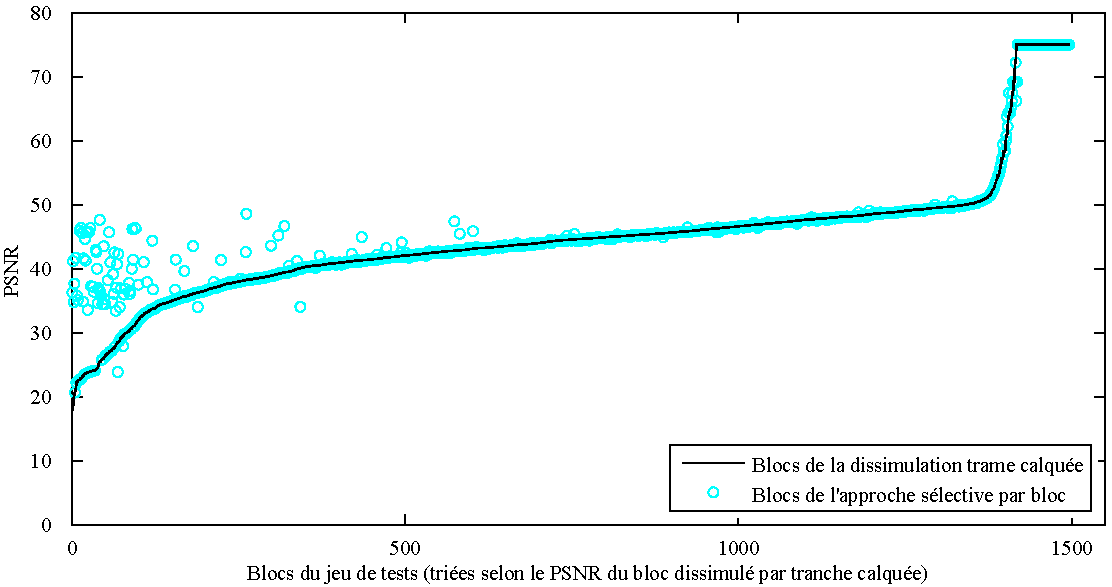
\includegraphics[width=0.97\linewidth]{Annexe/PlotSelectiveBlockDispersed1.pdf}
} \caption[]{PSNR des blocs de l'approche sélective par bloc par rapport au
calquage de trame. (Séquence=\textit{Akiyo}, FMO = Dispersé)}
\label{fig-ParSequenceDispersed1}
\end{figure}

\begin{figure} \fbox{ \centering
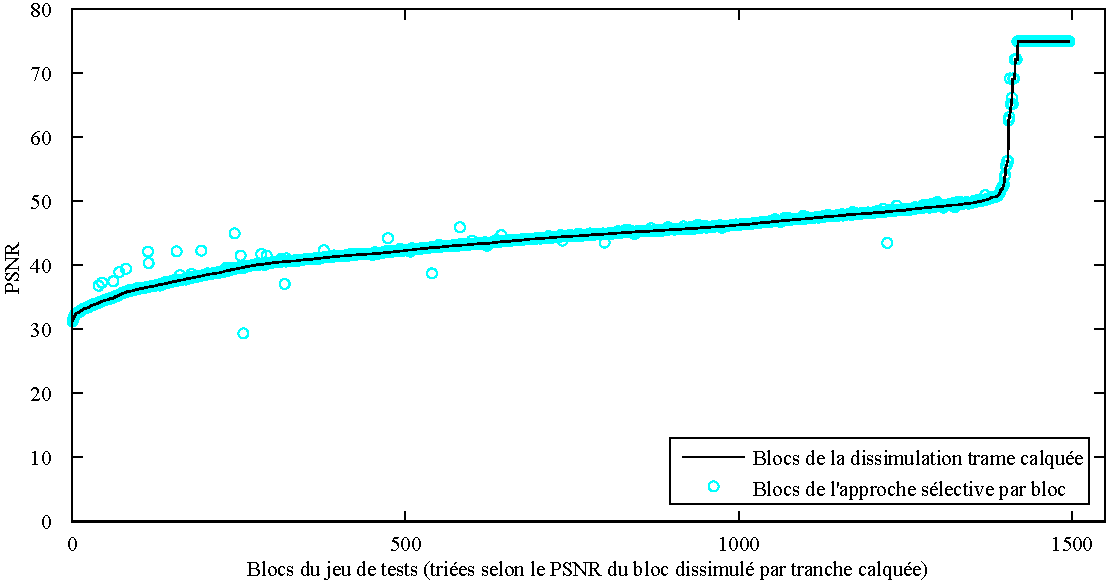
\includegraphics[width=0.97\linewidth]{Annexe/PlotSelectiveBlockInterleaved1.pdf}
} \caption[]{PSNR des blocs de l'approche sélective par bloc par rapport au
calquage de trame. (Séquence=\textit{Akiyo}, FMO = Entrelacé)}
\label{fig-ParSequenceInterleaved1}
\end{figure}

\begin{figure} \fbox{ \centering
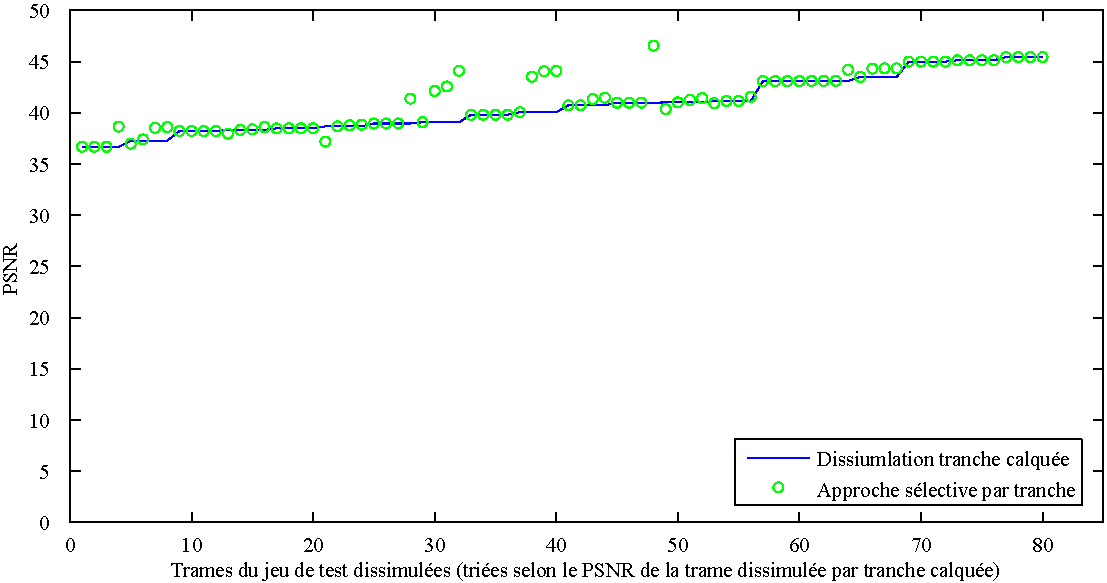
\includegraphics[width=0.97\linewidth]{Annexe/PlotSelectiveFrameDispersed1.pdf}
} \caption[]{PSNR des trames de l'approche sélective par trame par rapport au
calquage de trame. (Séquence=\textit{Akiyo}, FMO = Dispersé)}
\label{fig-ParSequenceFrameDispersed1}
\end{figure}

\begin{figure} \fbox{ \centering
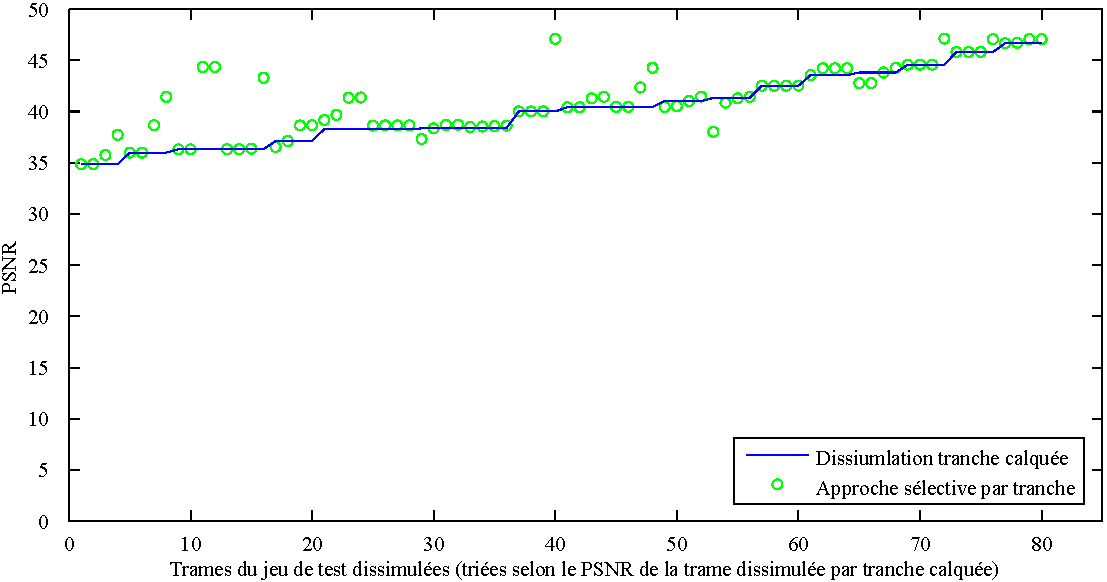
\includegraphics[width=0.97\linewidth]{Annexe/PlotSelectiveFrameInterleaved1.pdf}
} \caption[]{PSNR des trames de l'approche sélective par trame par rapport au
calquage de trame. (Séquence=\textit{Akiyo}, FMO = Entrelacé)}
\label{fig-ParSequenceFrameInterleaved1}
\end{figure}

\begin{figure} \fbox{ \centering
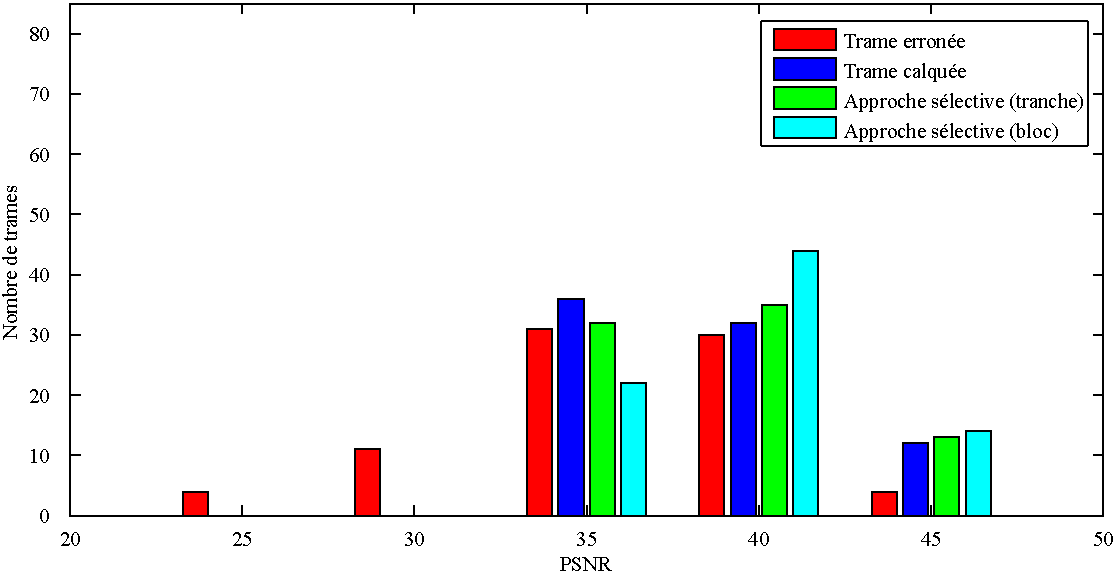
\includegraphics[width=0.97\linewidth]{Annexe/parSequenceDispersed1.pdf} }
\caption[]{Histogrammes des PSNR des trames, selon l'approche de dissimulation
utilisée. (Séquence=\textit{Akiyo}, FMO = Dispersé)}
\label{fig-ParSequenceDispersed1}
\end{figure}

\begin{figure} \fbox{ \centering
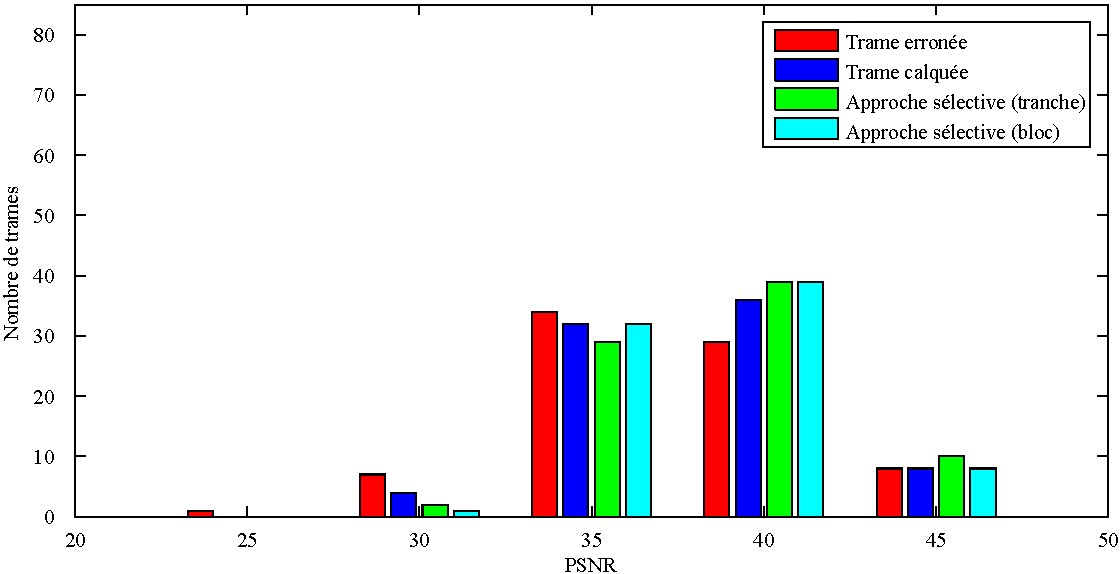
\includegraphics[width=0.97\linewidth]{Annexe/parSequenceInterleaved1.pdf} }
\caption[]{Histogrammes des PSNR des trames, selon l'approche de dissimulation
utilisée. (Séquence=\textit{Akiyo}, FMO = Entrelacé)}
\label{fig-ParSequenceInterleaved1}
\end{figure}

\FloatBarrier
\end{subsection}


\begin{subsection}{Séquence \textit{Carphone}}
\begin{table}
\caption[Résumé des résultats obtenus pour la séquence
\textit{Carphone}]{Résumé des résultats obtenus pour la séquence \textit{Carphone}.}
\centering
\begin{tabular}{| l | c | c |}
 \hline
 \multirow{2}{*}{\textbf{Approche}} & \textbf{PSNR Moyen}& \textbf{PSNR Moyen}\\
 &\textbf{dispersé (dB)}&\textbf{entrelacé (dB)}\\
 \hline
Encodée (sans erreur) & 41.40 & 41.20\\
Sélective par bloc (avec référence) & 36.57 & 34.81\\
Sélective par tranche (avec référence) & 35.69 & 34.13\\
Sélective par bloc & \textbf{35.84} &\textbf{33.80}\\
Sélective par tranche & \textbf{35.41} &\textbf{33.99}\\
Dissimulation tranche calquée & 34.63 &33.10\\
Trame corrompue & 33.71 &32.41\\
\hline
\end{tabular}
\end{table}

\begin{figure} \fbox{ \centering
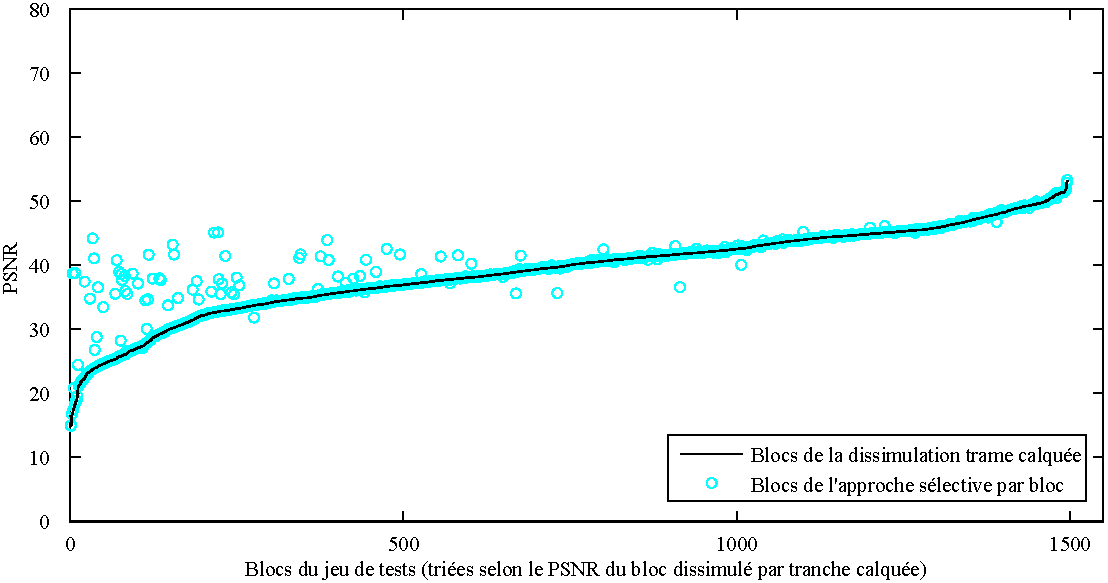
\includegraphics[width=0.97\linewidth]{Annexe/PlotSelectiveBlockDispersed4.pdf}
} \caption[]{PSNR des blocs de l'approche sélective par bloc par rapport au
calquage de trame. (Séquence=\textit{Carphone}, FMO = Dispersé)}
\label{fig-ParSequenceDispersed4}
\end{figure}

\begin{figure} \fbox{ \centering
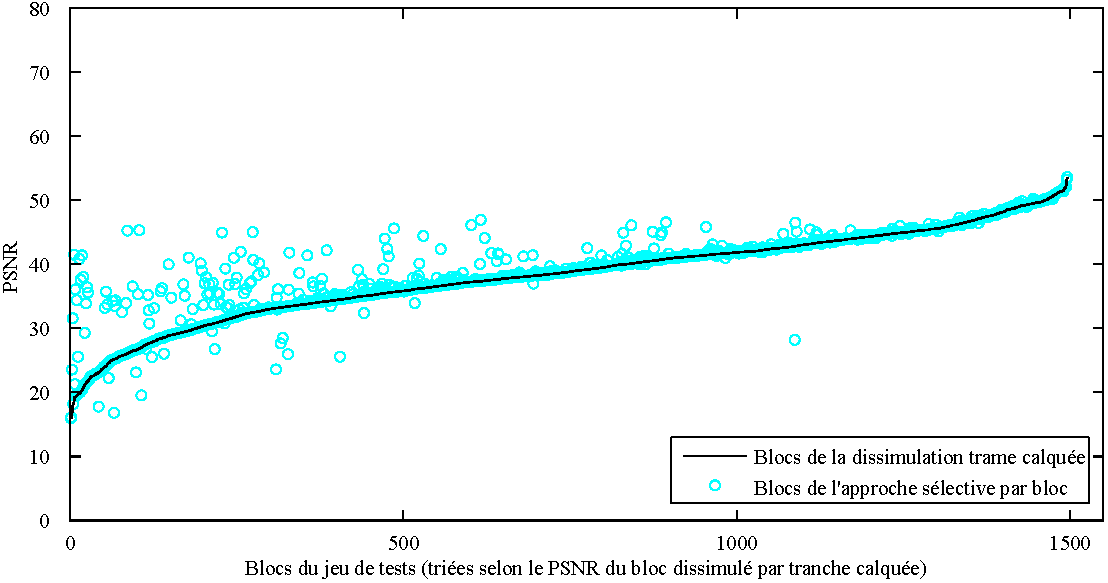
\includegraphics[width=0.97\linewidth]{Annexe/PlotSelectiveBlockInterleaved4.pdf}
} \caption[]{PSNR des blocs de l'approche sélective par bloc par rapport au
calquage de trame. (Séquence=\textit{Carphone}, FMO = Entrelacé)}
\label{fig-ParSequenceInterleaved4}
\end{figure}

\begin{figure} \fbox{ \centering
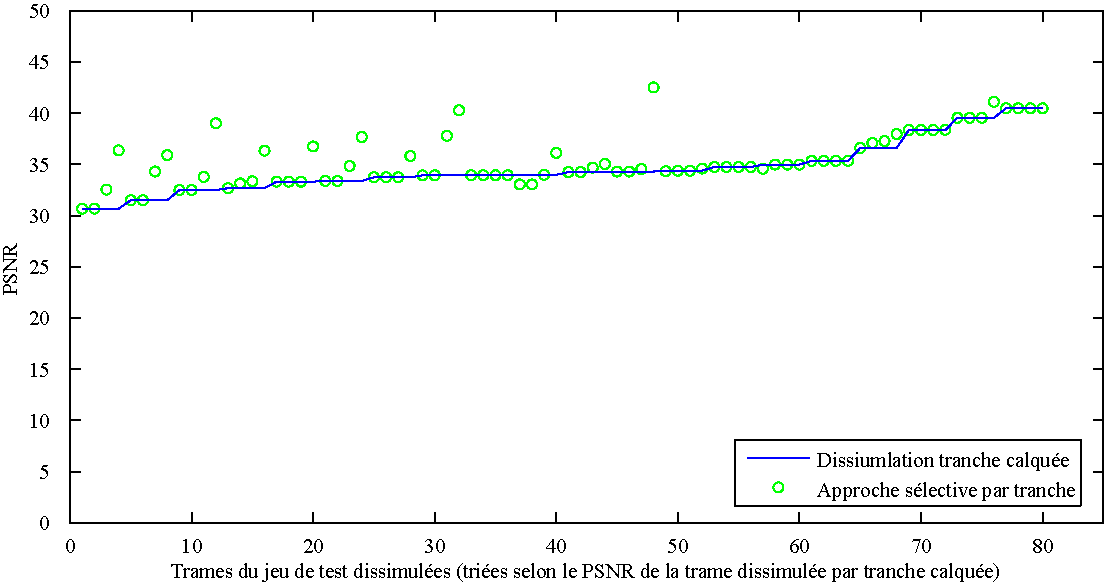
\includegraphics[width=0.97\linewidth]{Annexe/PlotSelectiveFrameDispersed4.pdf}
} \caption[]{PSNR des trames de l'approche sélective par trame par rapport au
calquage de trame. (Séquence=\textit{Carphone}, FMO = Dispersé)}
\label{fig-ParSequenceFrameDispersed4}
\end{figure}

\begin{figure} \fbox{ \centering
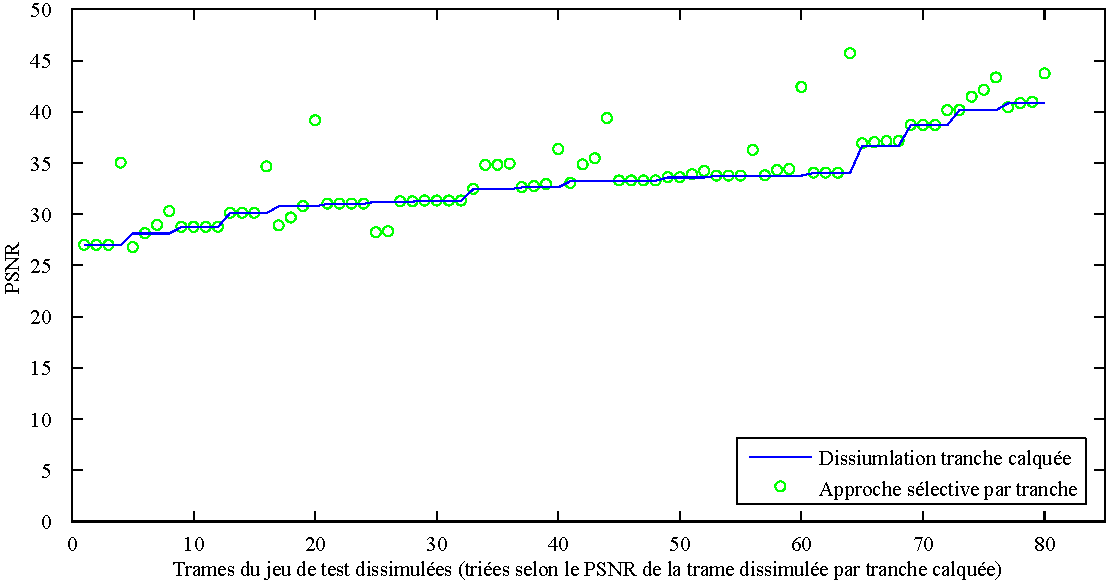
\includegraphics[width=0.97\linewidth]{Annexe/PlotSelectiveFrameInterleaved4.pdf}
} \caption[]{PSNR des trames de l'approche sélective par trame par rapport au
calquage de trame. (Séquence=\textit{Carphone}, FMO = Entrelacé)}
\label{fig-ParSequenceFrameInterleaved4}
\end{figure}

\begin{figure} \fbox{ \centering
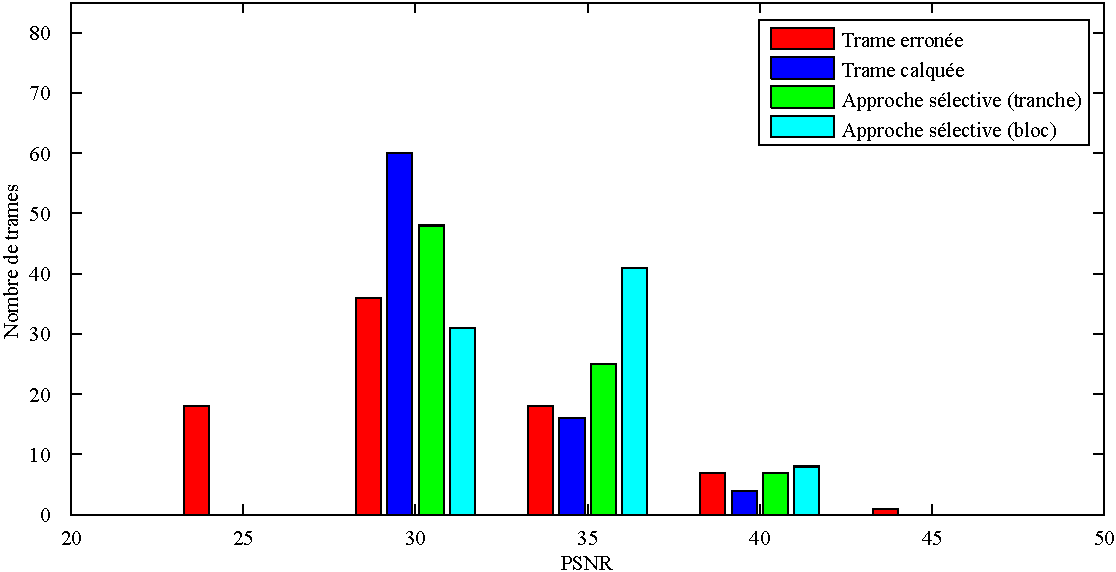
\includegraphics[width=0.97\linewidth]{Annexe/parSequenceDispersed4.pdf} }
\caption[]{Histogrammes des PSNR des trames, selon l'approche de dissimulation
utilisée. (Séquence=\textit{Carphone}, FMO = Dispersé)}
\label{fig-ParSequenceDispersed4}
\end{figure}

\begin{figure} \fbox{ \centering
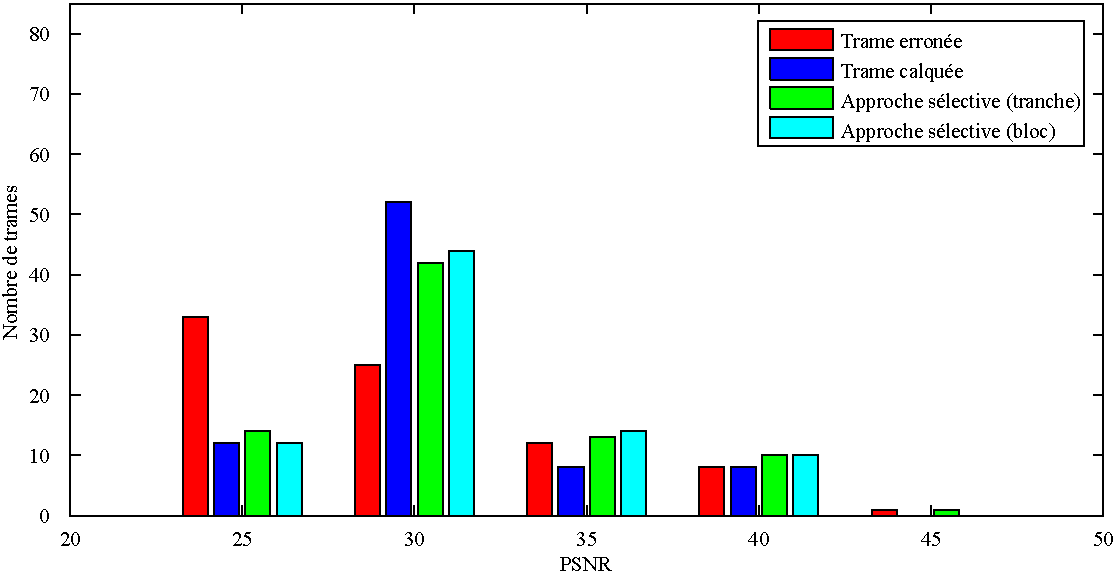
\includegraphics[width=0.97\linewidth]{Annexe/parSequenceInterleaved4.pdf} }
\caption[]{Histogrammes des PSNR des trames, selon l'approche de dissimulation
utilisée. (Séquence=\textit{Carphone}, FMO = Entrelacé)}
\label{fig-ParSequenceInterleaved4}
\end{figure}

\FloatBarrier
\end{subsection}

\begin{subsection}{Séquence \textit{Coastguard}}
\begin{table}
\caption[Résumé des résultats obtenus pour la séquence
\textit{Coastguard}]{Résumé des résultats obtenus pour la séquence
\textit{Coastguard}.}
\centering
\begin{tabular}{| l | c | c |}
 \hline
 \multirow{2}{*}{\textbf{Approche}} & \textbf{PSNR Moyen}& \textbf{PSNR Moyen}\\
 &\textbf{dispersé (dB)}&\textbf{entrelacé (dB)}\\
 \hline
Encodée (sans erreur) & 39.78 & 39.90\\
Sélective par bloc (avec référence) & 34.00 & 35.01\\
Sélective par tranche (avec référence) & 32.94 & 34.10\\
Sélective par bloc & \textbf{33.37} & \textbf{34.04}\\
Sélective par tranche & \textbf{32.79} & \textbf{33.98}\\
Dissimulation tranche calquée & 31.62 & 33.01\\
Trame corrompue & 30.51 & 31.21\\
\hline
\end{tabular}
\end{table}

\begin{figure} \fbox{ \centering
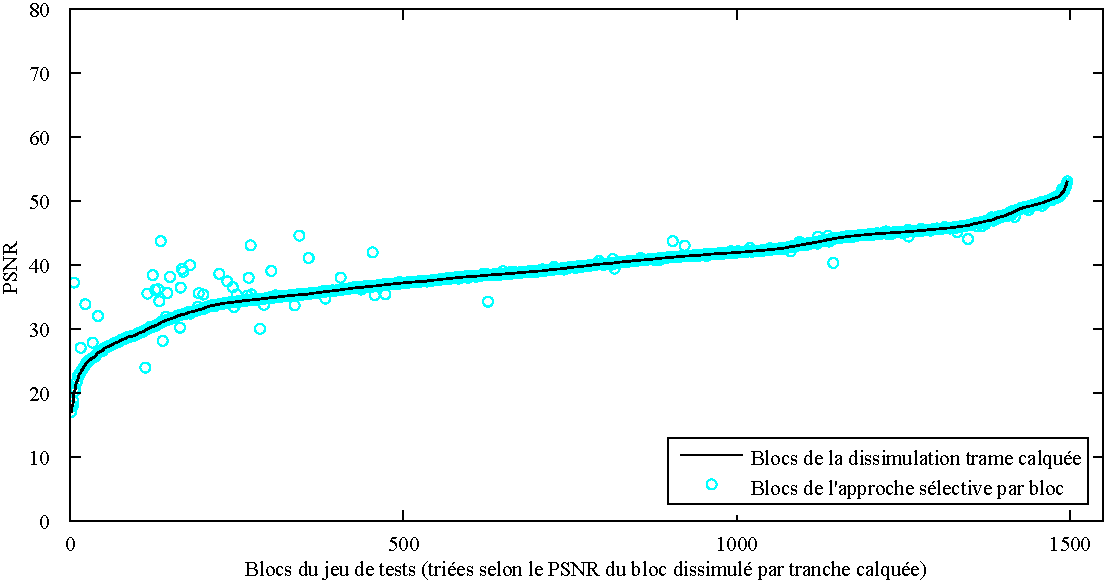
\includegraphics[width=0.97\linewidth]{Annexe/PlotSelectiveBlockDispersed6.pdf}
} \caption[]{PSNR des blocs de l'approche sélective par bloc par rapport au
calquage de trame. (Séquence=\textit{Coastguard}, FMO = Dispersé)}
\label{fig-ParSequenceDispersed6}
\end{figure}

\begin{figure} \fbox{ \centering
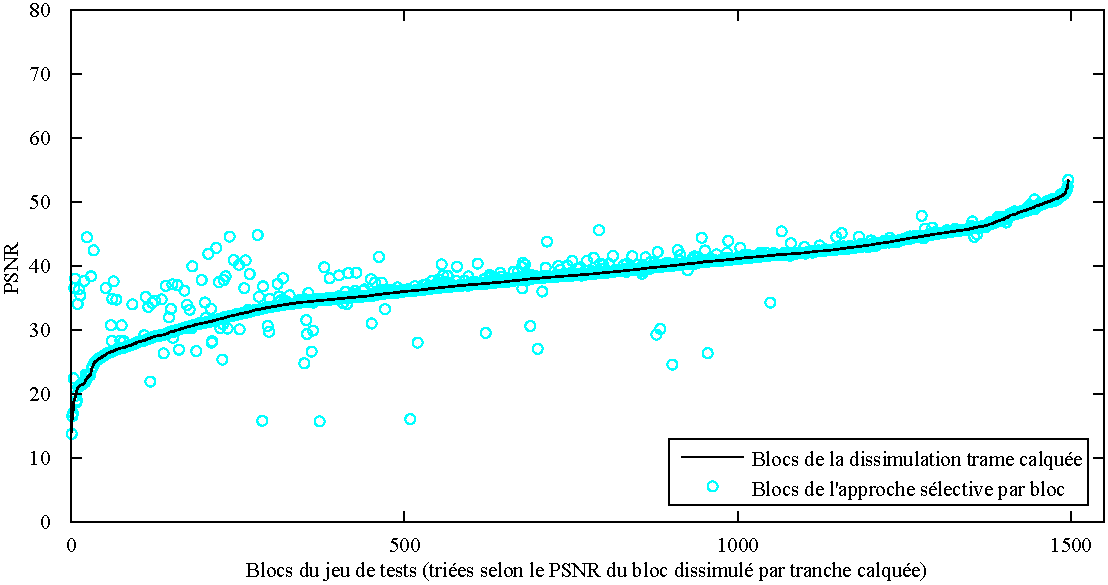
\includegraphics[width=0.97\linewidth]{Annexe/PlotSelectiveBlockInterleaved6.pdf}
} \caption[]{PSNR des blocs de l'approche sélective par bloc par rapport au
calquage de trame. (Séquence=\textit{Coastguard}, FMO = Entrelacé)}
\label{fig-ParSequenceInterleaved6}
\end{figure}

\begin{figure} \fbox{ \centering
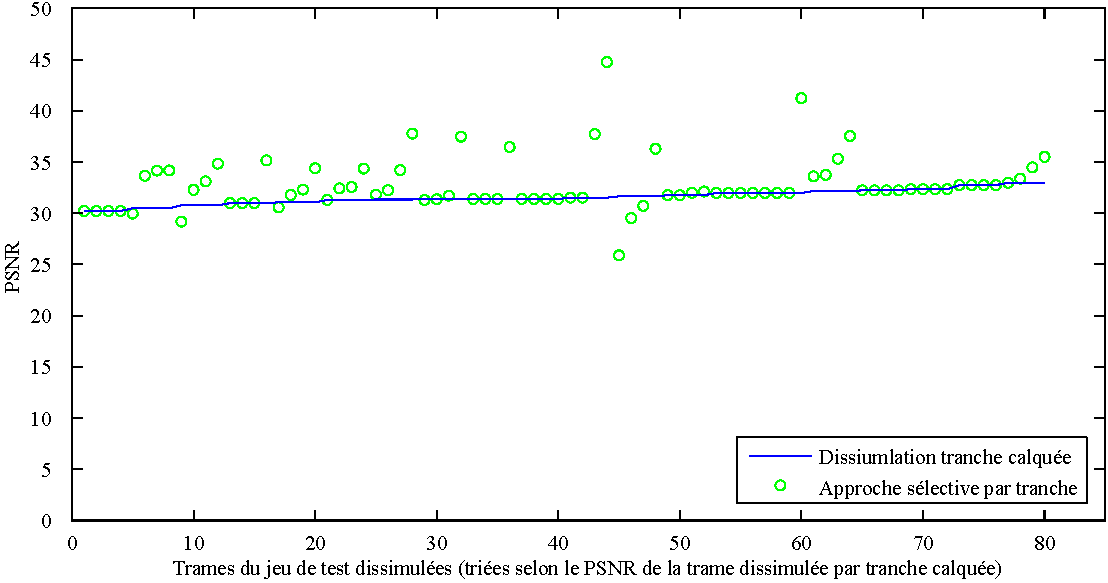
\includegraphics[width=0.97\linewidth]{Annexe/PlotSelectiveFrameDispersed6.pdf}
} \caption[]{PSNR des trames de l'approche sélective par trame par rapport au
calquage de trame. (Séquence=\textit{Coastguard}, FMO = Dispersé)}
\label{fig-ParSequenceFrameDispersed6}
\end{figure}

\begin{figure} \fbox{ \centering
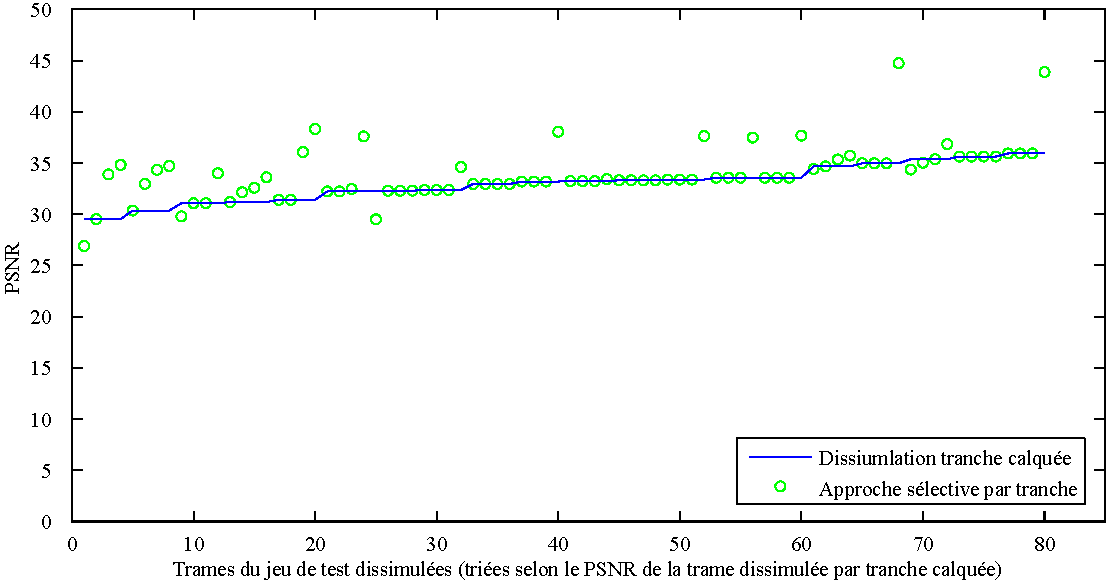
\includegraphics[width=0.97\linewidth]{Annexe/PlotSelectiveFrameInterleaved6.pdf}
} \caption[]{PSNR des trames de l'approche sélective par trame par rapport au
calquage de trame. (Séquence=\textit{Coastguard}, FMO = Entrelacé)}
\label{fig-ParSequenceFrameInterleaved6}
\end{figure}

\begin{figure} \fbox{ \centering
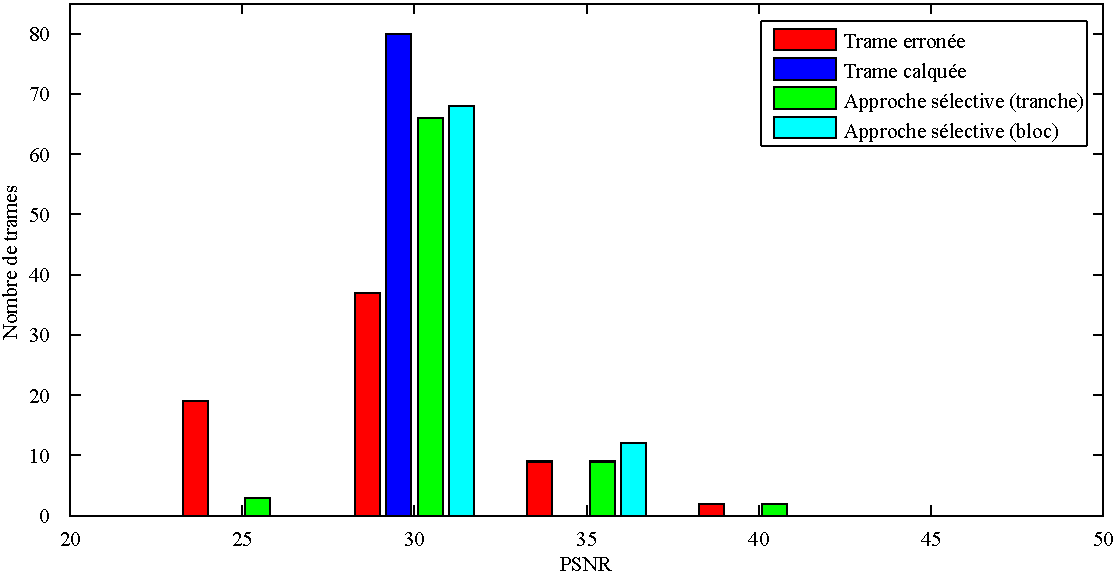
\includegraphics[width=0.97\linewidth]{Annexe/parSequenceDispersed6.pdf} }
\caption[]{Histogrammes des PSNR des trames, selon l'approche de dissimulation
utilisée. (Séquence=\textit{Coastguard}, FMO = Dispersé)}
\label{fig-ParSequenceDispersed6}
\end{figure}

\begin{figure} \fbox{ \centering
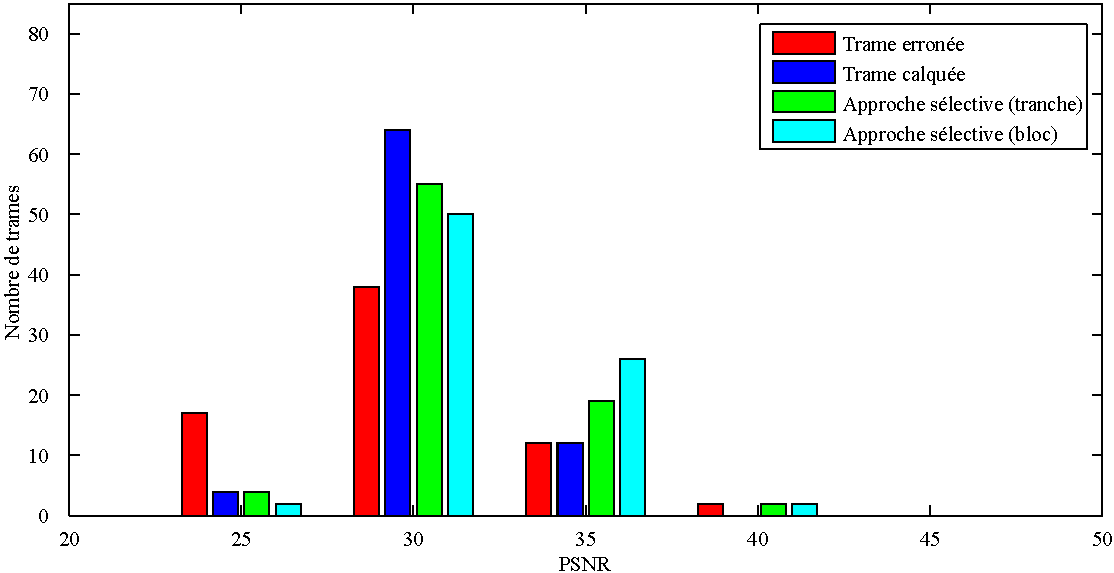
\includegraphics[width=0.97\linewidth]{Annexe/parSequenceInterleaved6.pdf} }
\caption[]{Histogrammes des PSNR des trames, selon l'approche de dissimulation
utilisée. (Séquence=\textit{Coastguard}, FMO = Entrelacé)}
\label{fig-ParSequenceInterleaved6}
\end{figure}

\FloatBarrier
\end{subsection}

\begin{subsection}{Séquence \textit{Foreman}}
\begin{table}
\caption[Résumé des résultats obtenus pour la séquence
\textit{Foreman}]{Résumé des résultats obtenus pour la séquence
\textit{Foreman}.}
\centering
\begin{tabular}{| l | c | c |}
 \hline
 \multirow{2}{*}{\textbf{Approche}} & \textbf{PSNR Moyen}& \textbf{PSNR Moyen}\\
 &\textbf{dispersé (dB)}&\textbf{entrelacé (dB)}\\
 \hline
Encodée (sans erreur) & 40.51 & 40.14\\
Sélective par bloc (avec référence) & 34.79 & 35.05\\
Sélective par tranche (avec référence) & 33.55 & 33.99\\
Sélective par bloc & \textbf{33.89} & \textbf{33.02}\\
Sélective par tranche & \textbf{33.45} & \textbf{32.70}\\
Dissimulation tranche calquée & 32.15 & 32.69\\
Trame corrompue & 31.87 & 31.72\\
\hline
\end{tabular}
\end{table}

\begin{figure} \fbox{ \centering
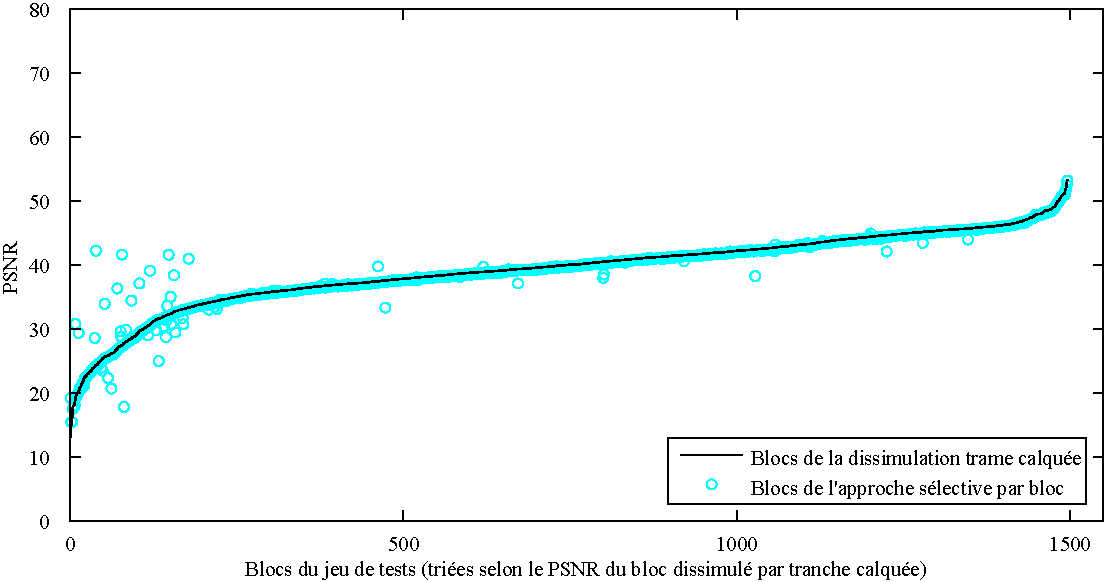
\includegraphics[width=0.97\linewidth]{Annexe/PlotSelectiveBlockDispersed8.pdf}
} \caption[]{PSNR des blocs de l'approche sélective par bloc par rapport au
calquage de trame. (Séquence=\textit{Foreman}, FMO = Dispersé)}
\label{fig-ParSequenceDispersed8}
\end{figure}

\begin{figure} \fbox{ \centering
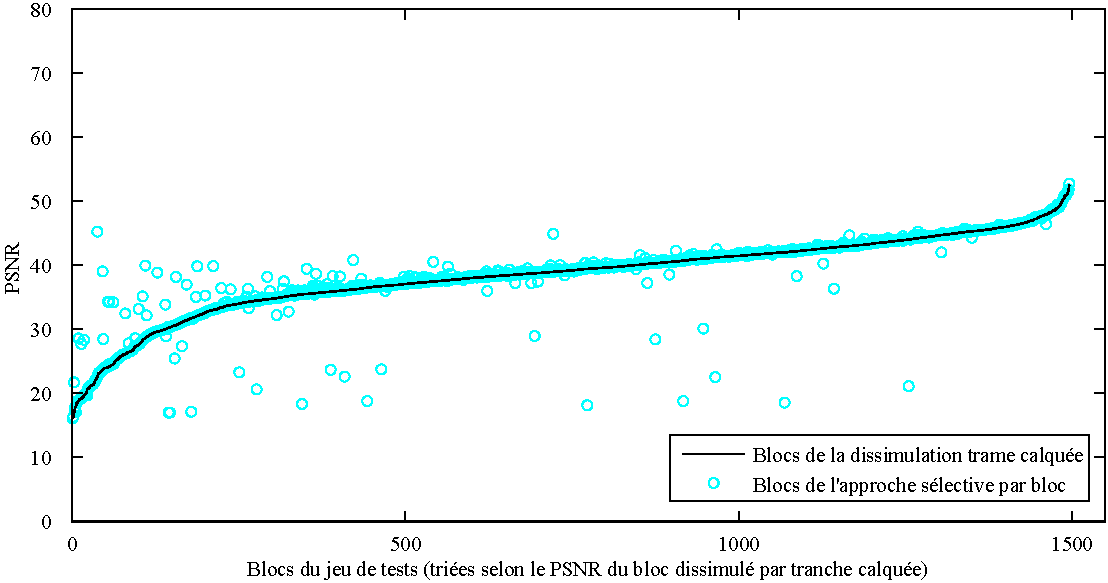
\includegraphics[width=0.97\linewidth]{Annexe/PlotSelectiveBlockInterleaved8.pdf}
} \caption[]{PSNR des blocs de l'approche sélective par bloc par rapport au
calquage de trame. (Séquence=\textit{Foreman}, FMO = Entrelacé)}
\label{fig-ParSequenceInterleaved8}
\end{figure}

\begin{figure} \fbox{ \centering
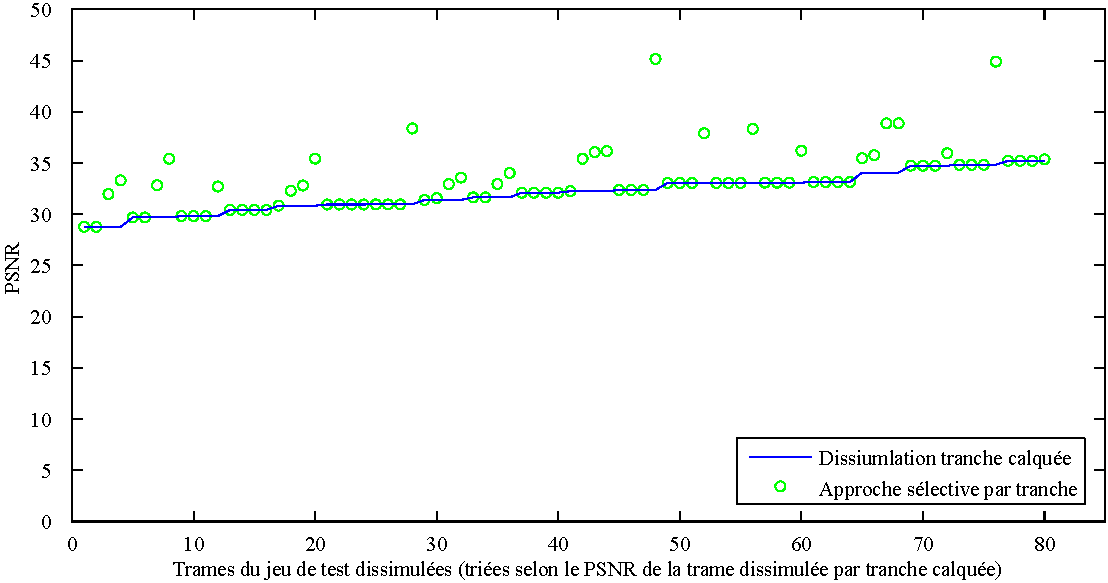
\includegraphics[width=0.97\linewidth]{Annexe/PlotSelectiveFrameDispersed8.pdf}
} \caption[]{PSNR des trames de l'approche sélective par trame par rapport au
calquage de trame. (Séquence=\textit{Foreman}, FMO = Dispersé)}
\label{fig-ParSequenceFrameDispersed8}
\end{figure}

\begin{figure} \fbox{ \centering
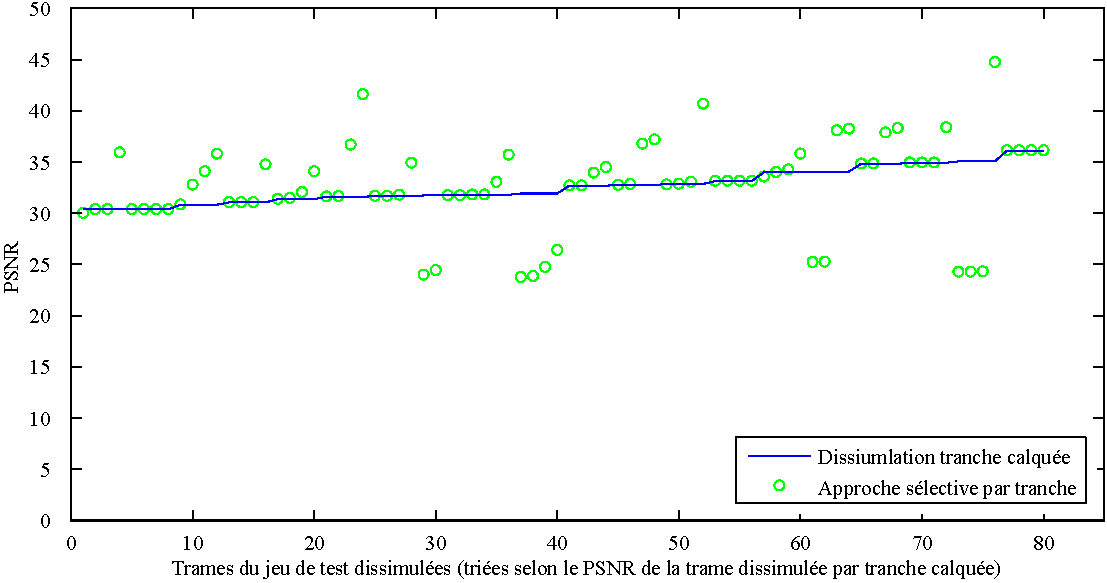
\includegraphics[width=0.97\linewidth]{Annexe/PlotSelectiveFrameInterleaved8.pdf}
} \caption[]{PSNR des trames de l'approche sélective par trame par rapport au
calquage de trame. (Séquence=\textit{Foreman}, FMO = Entrelacé)}
\label{fig-ParSequenceFrameInterleaved8}
\end{figure}

\begin{figure} \fbox{ \centering
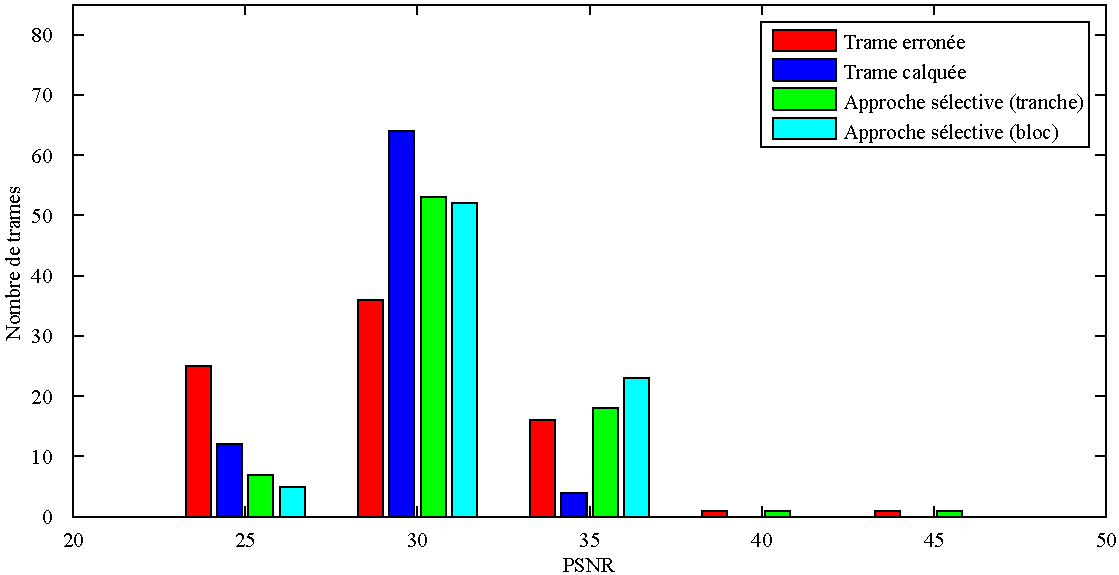
\includegraphics[width=0.97\linewidth]{Annexe/parSequenceDispersed8.pdf} }
\caption[]{Histogrammes des PSNR des trames, selon l'approche de dissimulation
utilisée. (Séquence=\textit{Foreman}, FMO = Dispersé)}
\label{fig-ParSequenceDispersed8}
\end{figure}

\begin{figure} \fbox{ \centering
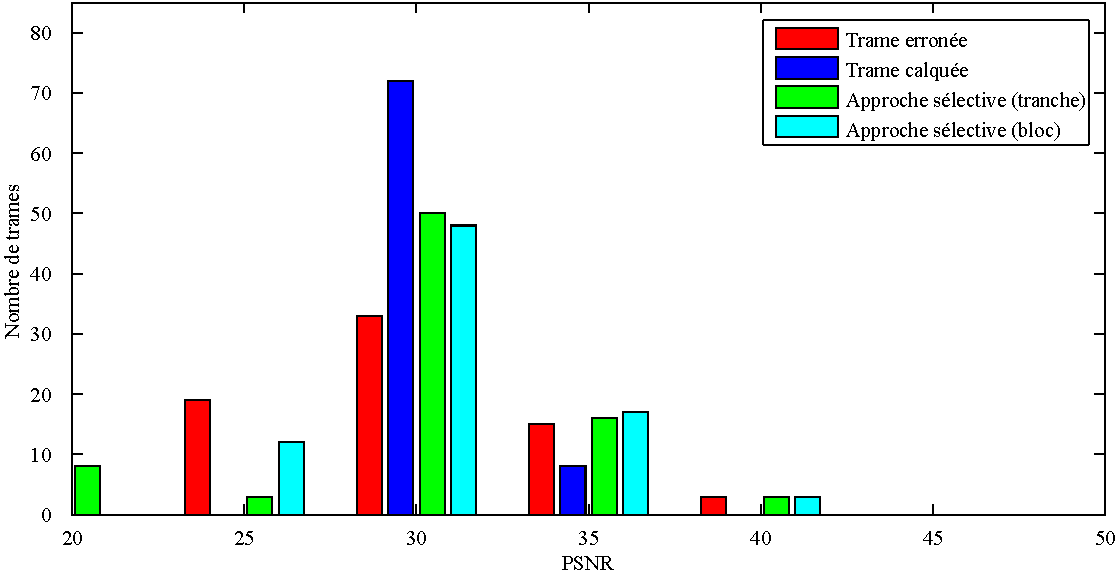
\includegraphics[width=0.97\linewidth]{Annexe/parSequenceInterleaved8.pdf} }
\caption[]{Histogrammes des PSNR des trames, selon l'approche de dissimulation
utilisée. (Séquence=\textit{Foreman}, FMO = Entrelacé)}
\label{fig-ParSequenceInterleaved8}
\end{figure}

\FloatBarrier
\end{subsection}

\FloatBarrier
\end{section}